\documentclass[14pt]{article}

\usepackage{fancyhdr}
\usepackage{extramarks}
\usepackage{amsmath}
\usepackage{amsthm}
\usepackage{amsfonts}
\usepackage{amssymb}
\usepackage{tikz}
\usepackage[plain]{algorithm}
\usepackage{algpseudocode}
\usepackage{enumitem}
\usepackage{relsize}
\usepackage{scrextend}
\usepackage{graphicx}

\usetikzlibrary{automata,positioning}

%
% Basic Document Settings
%

\topmargin=-0.45in
\evensidemargin=0in
\oddsidemargin=0in
\textwidth=6.5in
\textheight=9.0in
\headsep=0.25in

\linespread{1.1}

\pagestyle{fancy}
\lhead{\hmwkAuthorName}
\chead{\hmwkClass\ (\hmwkClassInstructor): \hmwkTitle}
\rhead{\firstxmark}
\lfoot{\lastxmark}
\cfoot{\thepage}

\renewcommand\headrulewidth{0.4pt}
\renewcommand\footrulewidth{0.4pt}

\setlength\parindent{0pt}

%
% Create Problem Sections
%

\newcommand{\enterProblemHeader}[1]{
    \nobreak\extramarks{}{Problem \arabic{#1} continued on next page\ldots}\nobreak{}
    \nobreak\extramarks{Problem \arabic{#1} (continued)}{Problem \arabic{#1} continued on next page\ldots}\nobreak{}
}

\newcommand{\exitProblemHeader}[1]{
    \nobreak\extramarks{Problem \arabic{#1} (continued)}{Problem \arabic{#1} continued on next page\ldots}\nobreak{}
    \stepcounter{#1}
    \nobreak\extramarks{Problem \arabic{#1}}{}\nobreak{}
}

\setcounter{secnumdepth}{0}
\newcounter{partCounter}
\newcounter{homeworkProblemCounter}
\setcounter{homeworkProblemCounter}{1}
\nobreak\extramarks{Problem \arabic{homeworkProblemCounter}}{}\nobreak{}

%
% Homework Problem Environment
%
% This environment takes an optional argument. When given, it will adjust the
% problem counter. This is useful for when the problems given for your
% assignment aren't sequential. See the last 3 problems of this template for an
% example.
%
\newenvironment{homeworkProblem}[1][-1]{
    \ifnum#1>0
        \setcounter{homeworkProblemCounter}{#1}
    \fi
    \section{Problem \arabic{homeworkProblemCounter}}
    \setcounter{partCounter}{1}
    \enterProblemHeader{homeworkProblemCounter}
}{
    \exitProblemHeader{homeworkProblemCounter}
}

%
% Homework Details
%   - Title
%   - Due date
%   - Class
%   - Section/Time
%   - Instructor
%   - Author
%


\newcommand{\hmwkClass}{CS 219}
\newcommand{\hmwkTitle}{Homework\ \#3}
\newcommand{\hmwkDueDate}{September 21, 2016}
\newcommand{\hmwkDueTime}{4:00pm}
\newcommand{\hmwkClassInstructor}{Dr. Egbert}
\newcommand{\hmwkAuthorName}{Matthew J. Berger}

%
% Title Page
%

\title{
    \vspace{2in}
    \textmd{\textbf{\hmwkClass:\ \hmwkTitle}}\\
    \normalsize\vspace{0.1in}\small{Due\ on\ \hmwkDueDate\ at \hmwkDueTime}\\
    \vspace{0.1in}\large{\textit{\hmwkClassInstructor}}
    \vspace{3in}
}

\author{\textbf{\hmwkAuthorName}}
\date{}

\renewcommand{\part}[1]{\textbf{\large Part \Alph{partCounter}}\stepcounter{partCounter}\\}

%
% Various Helper Commands
%

% Useful for algorithms
\newcommand{\alg}[1]{\textsc{\bfseries \footnotesize #1}}

% Alias for the Solution section header
\newcommand{\solution}{\textbf{\large Solution:}}

% Alias for answers
\newcommand{\answer}{\textbf{\large Answer: }}

\begin{document}

\maketitle

\pagebreak

\begin{homeworkProblem}
	\begin{itemize}
		\item[1.2.)] A.) On the IAS, what would the machine code instruction look like to load the contents of memory address 2 to the accumulator? \\
		
		\answer 
(with spaces between bytes for readability)
		
		\begin{table}[h]
		\def\arraystretch{1.5}%
		\hfil
			\begin{tabular}{|c|c|}
				\hline
				Opcode & Operand \\			
				\hline
				0000 0001 & 0000 0000 0010 \\
				\hline
			\end{tabular}
		\end{table}
		
		\item[     ] B.) How many trips to memory does the CPU need to make to complete this instruction during the instruction cycle? \\		
		
		\answer
		
		Initially, the CPU has to fetch the instruction at the program counter in memory. The instruction contains the address of the data to load. When executed, the memory is accessed in order to load the actual data located at that address in memory. This requires \underline{two trips} to memory during the instruction cycle.
		
		\item[1.3.)] On the IAS, describe in English the process that the CPU must undertake to read a value from memory and to write a value to memory in terms of what is put into the MAR, MBR, address bus, data bus, and control bus. \\
		
		\answer
		
		- To read a value from memory, the CPU places the address from the opcode in the MAR. Then the CPU will send a signal on the read control line to memory and puts the address on the address bus. After this, the memory will copy the contents of the memory location that was relayed by the data bus. Finally, the data is transferred to the MBR.
		
		- To write a value to memory, the CPU places the address from the opcode in the MAR. Then the cpu puts the data into the MBR. After, the CPU sends a signal on the write control line to memory and puts the address on the address bus, as well as the data on the data bus. Finally, the memory transfers the data on the data bus into the memory location relayed by the address bus.
		
		\pagebreak
		
		\item[1.4.)] Given the memory contents of the IAS computer shown below, \\
		\begin{table}[h]
		\def\arraystretch{1.5}%
		\hfil
			\begin{tabular}{|c|c|}
				\hline
				Address & Contents \\
				\hline
				08A & 010FA210FB \\
				08B & 010FA0F08D \\
				08C & 020FA210FB \\
				\hline
			\end{tabular}
		\end{table}
		
		Show the assembly language code for the program, starting at address 08A. Explain what this program does.
		
		\answer
		
		\begin{table}[h]
		\def\arraystretch{1.5}%
		\hfil
			\begin{tabular}{|c c l|}
				\hline
		 		\multicolumn{1}{|c|}{Address} &  \multicolumn{1}{|c|}{Instruction} & \multicolumn{1}{|c|}{Argument} \\
				\hline
				08A & LOAD &  M(0FA) \\
			        & STOR &  M(0FB) \\
			    \hline
				08B & LOAD &  M(0FA) \\								
				    & JUMP & +M(08D) \\
				\hline
				08C & LOAD & -M(0FA) \\
				    & STOR &  M(0FB) \\								
				\hline
			\end{tabular} 
		\end{table}
		
		This program stores the absolute value of the data at memory location 0x0FA into memory location 0x0FB.
		
		\item[1.5.)] In Figure 1.6, indicate the width, in bits, of each data path (e.g., between AC and ALU). \\
		
		\answer	
		\begin{itemize}
			\item Data paths to and from the MAR total to 12 bits.
			\item Data paths to and from the MBR total to 40 bits.
			\item All paths to and from the AC is 40 bits.
			\item All paths to and from the MQ is 40 bits.			
		\end{itemize}	
			
	\end{itemize}
\end{homeworkProblem}

\pagebreak

\begin{homeworkProblem}
	\begin{itemize}
		\item[2.2)] Consider two different machines, with two different instruction sets, both of which have a clock rate of \underline{200 MHz}. The following measurements are recorded on the two machines running a given set of benchmark programs:
		\begin{table}[h]
		\def\arraystretch{1.5}%
		\hfil
			\begin{tabular}{|l|c|c|}
			\hline
			Instruction Type & Instruction Count (millions) & Cycles Per Instruction \\
			\hline			
            & & \\
			Machine A & & \\
			\hline
			Arithmetic and Logic & 8 & 1 \\
			\hline
			Load and Store & 4 & 2 \\
			\hline
			Branch & 2 & 4 \\
			\hline
			Others & 4 & 3 \\
			\hline
			 & & \\
			Machine B & & \\
			\hline
			Arithmetic and Logic & 10 & 1 \\
			\hline
			Load and Store & 8 & 2 \\
			\hline
			Branch & 2 & 4 \\
			\hline
			Others & 4 & 3 \\
			\hline			
			\end{tabular}
		\end{table}
		
		A.) Determine the effective CPI, MIPS rate, and execution time for each machine.
	\item[    ]	B.) Comment on the results. \\
	
	\answer
	\begin{addmargin}[2em]{2em}
	\textsl{Machine A:}
		\begin{itemize}
			\item \( \mathlarger{CPI_A = \frac{\sum CPI_i \times I_i}{I_c} = \frac{((8\times1) + (4\times3) + (2\times4) + (4\times3)) \times 10^6}{(8+4+2+4) \times 10^6} \approx 2.22}\)
			\item \( \mathlarger{ MIPS_A = \frac{f}{CPI_A \times 10^6} = \frac{200 \times 10^6}{2.22 \times 10^6} = 90}\)
			\item \( \mathlarger{CPU_A = \frac{I_c \times CPI_A}{f}=\frac{18\times10^6\times2.22}{200\times10^6} = 0.20s}\)
		\end{itemize}
		
	\textsl{Machine B:}
		\begin{itemize}
			\item \( \mathlarger{CPI_B = \frac{\sum CPI_i \times I_i}{I_c} = \frac{((10\times1) + (8\times2) + (2\times4) + (4\times3)) \times 10^6}{(10+8+2+4) \times 10^6} \approx 1.92}\)
			\item \( \mathlarger{ MIPS_B = \frac{f}{CPI_B \times 10^6} = \frac{200 \times 10^6}{1.92 \times 10^6} = 104}\)
			\item \( \mathlarger{CPU_B = \frac{I_c \times CPI_B}{f}=\frac{24\times10^6\times1.92}{200\times10^6} = 0.23s}\)
		\end{itemize}
	\end{addmargin}
	
	Machine B has a higher MIPS than Machine A, but it takes a slightly longer CPU time to execute the same set of benchmark instructions and is therefore slightly less efficient than Machine A.
	
	\pagebreak
	
		\item[2.4)] Four benchmark programs are executed on three computers with the following results:
		
		\begin{table}[h]
		\def\arraystretch{1.5}%
		\hfil
			\begin{tabular}{|l|c|c|c|}
				\hline
		 		& Computer A & Computer B & Computer C \\
				\hline
				Program 1 & 1 & 10 & 20 \\
				\hline
				Program 2 & 1000 & 100 & 20 \\
				\hline
				Program 3 & 500 & 1000 & 50 \\
				\hline				
				Program 4 & 100 & 800 & 100 \\								
				\hline
			\end{tabular} 
		\end{table}
		
The table shows the execution time in seconds, with 100,000,000 instructions executed in each of the four programs. Calculate the MIPS values for each computer for each program. Then calculate the arithmetic and harmonic means assuming equal weights of the four programs, and rank the computers based on arithmetic and harmonic mean.

		\item[] \hfil MIPS rate is \(\mathlarger{MIPS = \frac{I_c}{T \times 10^6}}\)
		\item[] \hfil Arithmetic mean is \(\mathlarger{R_A = \frac{1}{M}\sum_{i=1}^{m}R_i}\)
		\item[] \hfil Harmonic mean is \(\mathlarger{R_H = \frac{m}{\sum_{i=1}^{m}\frac{1}{R_i}}}\)
		
		With the MIPS formula:
		
		$MIPS = \frac{I_c}{T \times 10^6} = \frac{100,000,000}{T \times 10^6}=\frac{100}{T}$
		
		Thus, the MIPS values are as follows:
		
		\begin{table}[h]
		\def\arraystretch{1.5}%
		\hfil
			\begin{tabular}{|l|c|c|c|}
				\hline
		 		& Computer A & Computer B & Computer C \\
				\hline
				Program 1 & 100 & 10 & 5 \\
				\hline
				Program 2 & 0.1 & 1 & 5 \\
				\hline
				Program 3 & 0.2 & 0.1 & 2 \\
				\hline				
				Program 4 & 2 & 0.125 & 1 \\								
				\hline
			\end{tabular} 
		\end{table}
		
		\begin{table}[h]
		\def\arraystretch{1.5}%
		\hfil
			\begin{tabular}{|l|c|c|}
				\hline
		 		& Arithmetic Mean & Rank\\
				\hline
				Computer A & 25.575 & 1 \\
				\hline
				Computer C & 3.25   & 2 \\
				\hline
				Computer B & 2.80   & 3 \\
				\hline
			\end{tabular} 
			\begin{tabular}{|l|c|c|}
				\hline
		 		& Harmonic Mean & Rank\\
   				\hline
				Computer C & 2.1  & 1 \\	
				\hline
				Computer A & 0.25 & 2 \\
				\hline
				Computer B & 0.21 & 3 \\
				\hline
			\end{tabular} 
		\end{table}
	\end{itemize}
\end{homeworkProblem}

\pagebreak

\begin{homeworkProblem}

Download the Simulated Computer zip and pdf files from the Simulated Computer Folder on Canvas. Unzip and install the executable file on your own computer. The provided version actually runs on an ATARI 800 computer. An emulator for the ATARI 800 is included in the zip file. The program to execute after un-zipping is 'ATARI800Win.exe'. The first time you run the emulator you should click on \linebreak File $\rightarrow$ Autoboot Image $\rightarrow$ Simulated Computer II.atr. After this, when you execute the emulator the Simulated Computer program should automatically start. The provided PDF is the user's manual for the simulated computer.

After you review Appendices II, III, and IV of the user's manual, write assembly language programs for the following three exercises. Include screen shots and separate program listings for exercises.

Program listings should have one line per instruction/address as follows:

		\begin{table}[h]
		\def\arraystretch{1.5}%
		\hfil
			\begin{tabular}{|c c c|}
				\hline
		 		\multicolumn{1}{|c|}{Line Number} &  \multicolumn{1}{|c|}{Instruction}  & \multicolumn{1}{|c|}{Comments} \\
				\hline
				03 & LDA15 & // Load the value 15 into the accumulator \\
				\hline
			\end{tabular} 
		\end{table}
		
\pagebreak
		
	\begin{itemize}
	\section{ Evaluating Algebraic Expressions}
	\item[3.1)]	Those of you who have stuided algebra may recall that you were occasionally required to calculate the value of an expression when particular values are substituted for variables. For example, the expression $7X$ is equal to $14$ if $X = 2$. The value is $42$ if $X = 6$. The value of the expression $3X - 5$ is 13 if you substitute $6$ for $X$. (Note: 3X means 3 times X.)
	
	Write a computer program which will evaluate the expression: $7X - 8$. Check your program by running it and inputting the numbers given below.
	
		\begin{table}[h]
		\def\arraystretch{1.5}%
		\hfil
			\begin{tabular}{|c|c|}
				\hline
		 		Input & Output \\
				\hline
				3 & 13 \\
				\hline
				43 & 293 \\				
				\hline
			\end{tabular} 
		\end{table}
		
	\solution
	
		\begin{table}[h]
		\def\arraystretch{1.5}%
		\hfil
			\begin{tabular}{|c l l|}
				\hline
		 		\multicolumn{1}{|c|}{Line Number} &  \multicolumn{1}{|c|}{Instruction}  & \multicolumn{1}{|c|}{Comments} \\
				\hline
				00 & INP14 & // Input a value to location 14 \\
				01 & LDA14 & // Load the value at location 14 into the Accumulator \\
				02 & MUL12 & // Multiply the value in the Accumulator by the value at location 12 \\
				03 & SUB13 & // Substract the value in the Accumulator by the value at location 13 \\					
				04 & STA14 & // Store the value in the Accumulator at location 14 \\
				05 & OUT14 & // Output the value at location 14 \\
				06 & STP   & // HALT \\	
				\hline
			\end{tabular} 
		\end{table}
		
		A screenshot of this program can be found on the next page:
		
\pagebreak
		\centerline{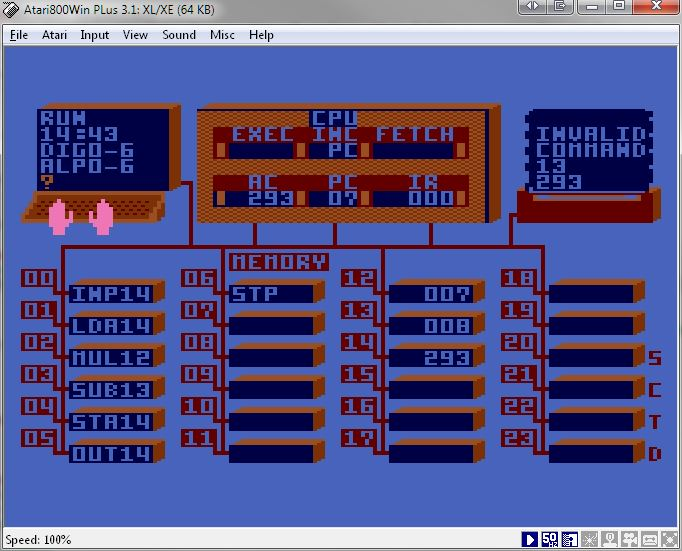
\includegraphics{expressionevaluation.jpg}}
\pagebreak

	\section{Number Sequences}
	\item[3.2)]	A number sequence is a series of numbers that follow a particular "rule", or pattern, as they go from one to the next. For example, the sequence:\\\\
	(a) 3, 6, 12, 24, 48, 96, etc. \\\\
	uses the rule "multiply by 2". Can you guess the rule for the following sequence? \\\\
	(b) 2, 5, 11, 23, 47, 95, etc. \\\\
	(It is "times 2 then add 1".) \\
	
	Once you know the rule for a sequence, you can write a program which will output that sequence. First, write programs that output sequences (a) and (b).
	
	Then write a program that outputs the Fibonacci sequence: \\\\
	(c) 1, 1, 2, 3, 5, 8, 13, 21, 34, etc. \\
	
		\solution\ \ \large{Sequence A}
		
		\begin{table}[h]
		\def\arraystretch{1.5}%
		\hfil
			\begin{tabular}{|c l l|}
				\hline
		 		\multicolumn{1}{|c|}{Line Number} &  \multicolumn{1}{|c|}{Instruction}  & \multicolumn{1}{|c|}{Comments} \\
				\hline
				00 & LDA14 & // Load the loop counter's current value - Initialized to 6 in memory \\
				01 & SUB15 & // Subtract one from the loop counter \\
				02 & STA14 & // Store the decremented loop counter at the same address it was loaded from \\
				03 & LDA12 & // Load the current value in the sequence \\				
				04 & OUT12 & // Output the current value \\
				05 & MUL13 & // Multiply the current value by 2 - Address 13 is preinitialized to 2 in memory \\
				06 & STA12 & // Store the current value, overwriting the original location \\	
				07 & LDA14 & // Load the loop counter's current value into the accumulator \\	
				08 & SKP4  & // Skip the next instruction if the value in the Accumulator is less than or equal to 0 \\	
				09 & JMP1  & // Jump to address 01 \\	
				10 & STP   & // HALT \\													
				\hline
			\end{tabular} 
		\end{table}
	
		A screenshot of this program can be found on the next page:
		
\pagebreak
		\centerline{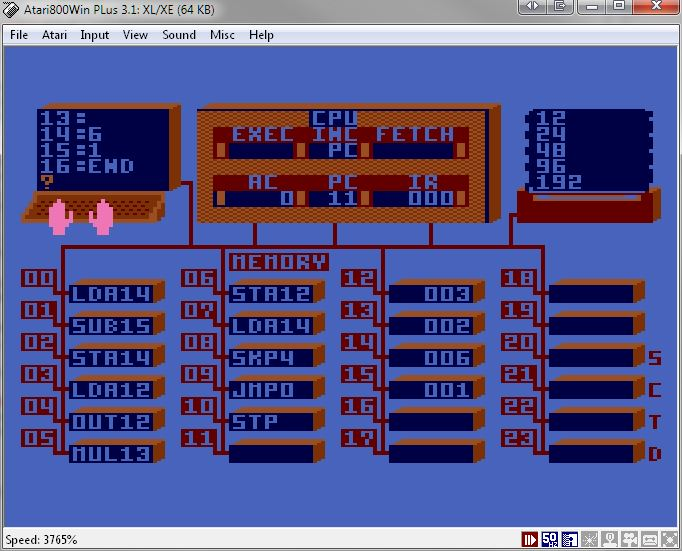
\includegraphics{sequence1.jpg}}
\pagebreak

		\solution\ \ \large{Sequence B}
		
		\begin{table}[h]
		\def\arraystretch{1.5}%
		\hfil
			\begin{tabular}{|c l l|}
				\hline
		 		\multicolumn{1}{|c|}{Line Number} &  \multicolumn{1}{|c|}{Instruction}  & \multicolumn{1}{|c|}{Comments} \\
				\hline
				00 & LDA16 & // Load the loop counter's current value - Initialized to 6 in memory \\
				01 & SUB17 & // Subtract one from the loop counter \\
				02 & STA16 & // Store the decremented loop counter at the same address it was loaded from \\
				03 & LDA14 & // Load the current value in the sequence \\				
				04 & OUT14 & // Output the current value to the screen \\
				05 & MUL15 & // Multiply the current value by 2 - Address 15 is preinitialized to 2 in memory \\
				06 & ADD17 & // Add 1 to the current value \\	
				07 & STA14 & // Store the current value, overwriting the original location \\	
				08 & LDA16 & // Load the loop counter's current value into the accumulator \\	
				09 & SKP4  & // Skip the next instruction if the value in the Accumulator is less than or equal to 0 \\	
				10 & JMP1  & // Jump to address 01 \\													
				11 & STP   & // HALT \\
				\hline
			\end{tabular} 
		\end{table}
	
		A screenshot of this program can be found on the next page:
		
\pagebreak
		\centerline{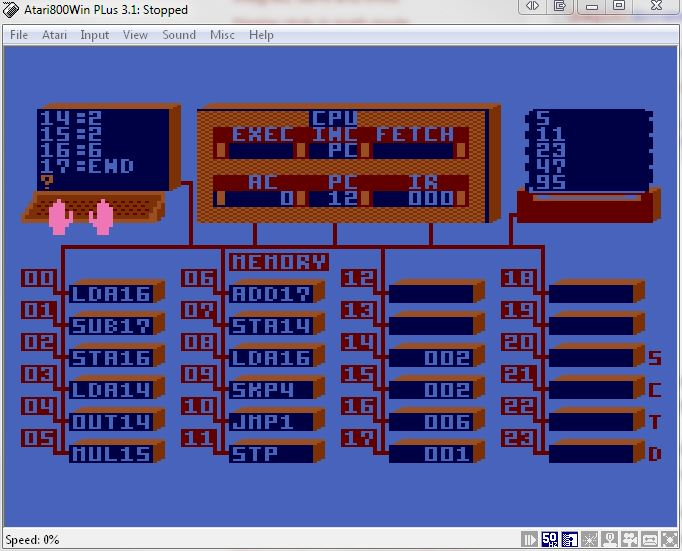
\includegraphics{sequence2.jpg}}
\pagebreak

		\solution\ \ \large{Sequence C}
		
		\begin{table}[h]
		\def\arraystretch{1.5}%
		\hfil
			\begin{tabular}{|c l l|}
				\hline
		 		\multicolumn{1}{|c|}{Line Number} &  \multicolumn{1}{|c|}{Instruction}  & \multicolumn{1}{|c|}{Comments} \\
				\hline
				00 & LDA16 & // Load the loop counter's current value - Initialized to 6 in memory \\
				01 & SUB17 & // Subtract one from the loop counter \\
				02 & STA16 & // Store the decremented loop counter at the same address it was loaded from \\
				03 & OUT15 & // Output current value in the sequence \\				
				04 & LDA14 & // Load the next sequence value from location 14 into the Accumulator \\
				05 & ADD15 & // Add the prior sequence value to the Accumulator \\
				06 & STA14 & // Store the current value at the 'next value' address \\	
				07 & ADD15 & // Add the previous value to the Accumulator value to get the next value in the sequence \\	
				08 & STA15 & // Store the Accumulated value, this becomes the 'previous value' in the next iteration \\	
				09 & OUT14 & // Output the current value. Both previous and next value are output each iteration. \\	
				10 & LDA16 & // Load the loop counter's current value \\													
				11 & SKP4  & // Skip the next instruction if the value in the Accumulator is less than or equal to 0 \\	
				12 & JMP1  & // Jump to address 01 \\
				13 & STP   & // HALT \\
				\hline
			\end{tabular} 
		\end{table}
	
		A screenshot of this program can be found on the next page:
		
\pagebreak
		\centerline{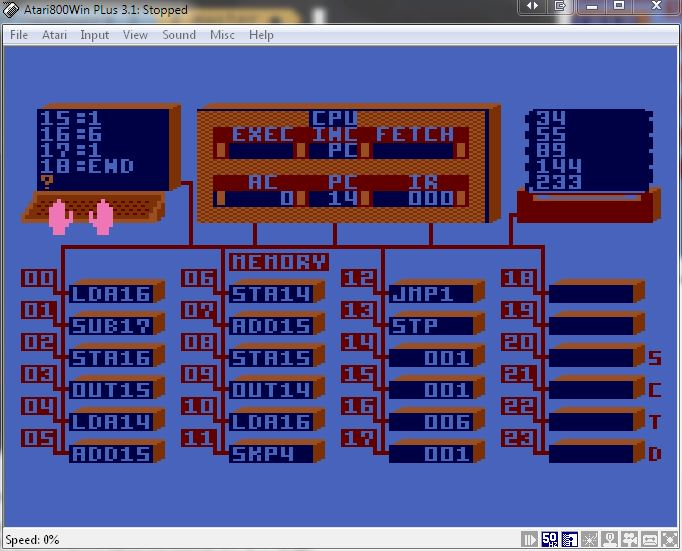
\includegraphics{sequence3.jpg}}
\pagebreak

	\section{A Decision Maker}
	\item[3.3)]	Write a program that uses an INP instruction. If the number that you INPut is positive or zero, have your program OUTput the number 1. If the number that you INPut is negative, have the program OUTput the number zero.
	
		\solution\ \ \large{Sequence C}
		
		\begin{table}[h]
		\def\arraystretch{1.5}%
		\hfil
			\begin{tabular}{|c l l|}
				\hline
		 		\multicolumn{1}{|c|}{Line Number} &  \multicolumn{1}{|c|}{Instruction}  & \multicolumn{1}{|c|}{Comments} \\
				\hline
				00 & INP14 & // Input a number to location 14 \\
				01 & LDA14 & // Load the value at location 14 into the Accumulator \\
				02 & SKP5  & // Skip the next instruction if the value in the Accumulator is positive \\
				03 & OUT13 & // Output the value stored at location 13 - Initialized to 0 \\				
				04 & SKP1  & // Skip the next instruction if the value in the Accumulator is positive \\
				05 & OUT12 & // Output the value stored at location 12 - Initialized to 1 \\
				06 & STP   & // HALT \\	
				\hline
			\end{tabular} 
		\end{table}
	
		A screenshot of this program can be found on the next page:
		
\pagebreak
		\centerline{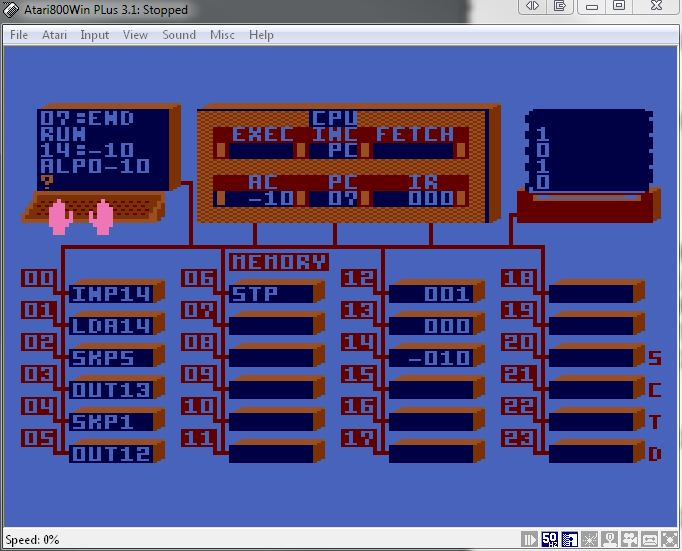
\includegraphics{decisionmaker.jpg}}
	\end{itemize}
\end{homeworkProblem}

\end{document}
